\chapter{General description}
This chapter describes general aspects of the application to be created as requested by the client.

\section{Product perspective} % application -> web service?
The aim of this project is to deliver an application that allows the user to visualise the mixing of fluids. To accomplish this, the user should be able to specify initial parameters, such as the shape of the mixer, in an intuitive and attractive user interface. These parameters should be set on a client device, which will send them to a server (owned by our Client) to compute the displacement of the fluids. When this server has computed the resulting fluid concentration distribution, this distribution is sent back to the client device, where it can be visualised.

A similar project was initiated around eleven years ago. The result of this project was a \textsc{Matlab} implementation that achieved a similar goal as our project. However, its user interface is outdated by now, and it is impossible to comfortably use this solution on a mobile device. Part of this original solution was a \textsc{Fortran} implementation for the displacement of the fluids. This implementation is still available, and we are to use it as a black box which can compute the resulting concentration distribution given some constraints.

\section{General capabilities}
This chapter describes the general properties our application should have. Firstly, the mixing constraints are described, detailing the parameters the user should set in order to be able to compute the displacement of fluids. Secondly, we describe additional capabilities of the application, such as storage and portability.

\subsection{Mixing constraints}\label{mixingconstraints}
As mentioned before, the application should be able to visualise the mixing of fluids. There are a number of constraints to be specified on the client device to accomplish this.

The first constraint is the geometry of the mixer. There are four kinds of geometries in total: rectangle, square, circle, and \emph{Journal Bearing}. We will start by implementing support for rectangular geometries, and we will implement more geometries if time permits.

The second constraint concerns the characteristics of the mixer. These influence the flow of the fluids. Stored in the server are multiple pre-computed matrices which each specify one set of mixer characteristics. Whenever these characteristics are changed, a different matrix must be used. Each geometry has its own set of possible characteristics and hence its own set of matrices.

The third constraint concerns parameters applicable to the mixer and the mixing protocol. Available parameters are determined by the type of mixer defined in the second constraint. For example, a rectangular mixing geometry has two walls that can be moved. The step parameter $D$ indicates the amount of time the wall should move, and is fixed for the entire protocol. Possible values for $D$ are 4, 2, 1, 0.5, 0.25 and 0.1, which can be combined to create other values. For example, a value of 6.2 can be achieved by setting $D=4+2+0.1+0.1$. The user can specify whether a complete protocol should be executed a number of times, or to only execute one step at a time. For a protocol for a rectangular geometry, the user can choose to move each of the two walls for $D$ time units at a time. The user can move the top wall to the right ($T$), the bottom wall to the left ($B$), or one of those walls to the other direction ($-T$ or $-B$).

The fourth constraint is the initial concentration distribution of the fluids. This can be specified either by loading an existing initial distribution, or by drawing on a canvas that has the shape of the selected mixer. The only supported method of drawing is free-form drawing, described as follows: to draw on the canvas, the user should first select one of two possible colors, namely black or white. Then, the user should select either a square or a circle for drawing. The final choice is the size of the shape that will be used to draw. For example, a large size is useful for quickly colouring large parts of the screen, and a small size is suitable for accurately colouring details. After choosing these parameters, the user can tap on or drag over the screen, to indicate where the selected fluid should be placed.

\subsection{Additional capabilities}
The main user interface is intended to be run on a mobile device, such as an iPhone. As we are creating a cross-platform solution, the application should also run on other devices, such as PCs and laptops. However, we are not actively supporting such devices. On the chosen client device, the constraints mentioned in Section \ref{mixingconstraints} should be specified. When the initial parameters have been set, the computation of the new concentration distribution is offloaded to the Client's server. After each iteration of the mixing protocol, the result -- along with a metric indicating the performance of the mixer -- is sent back to the client device to be shown to the user via a two-dimensional image of the fluid concentration distribution.

A history of past simulations is stored on the device to compare multiple runs. The result of runs should be exportable to commonly-used vector graphics files with support for alpha channels (to realise transparency). An additional capability might involve saving of entire runs -- hence including intermediate results -- as an animation.

After each result is received and visualised by the client device, the user has the choice of continuing with the received concentration distribution, or to reset the concentration distribution to a completely white concentration distribution.

\section{General constraints}
The user interface should be suitable for mobile devices, so it will be easy to share the visualised results with other people, and to quickly try out new ideas for mixers wherever the user may be.

We assume that the server can compute the displacement of fluids reasonably fast, so the visualisation of results can be handled quickly. When the new concentration distribution has been computed, this concentration distribution is sent back to the client device along with a metric to indicate the performance of the mixer.

As we do not want to be locked to one specific type of device, we have chosen to design a cross-platform solution. While this means that desktop PCs should also be able to run the application, we do not actively support such devices. We will instead concentrate on mobile devices.

As mentioned before, it should be possible to save mixing runs on the client device for later reference. For each saved run, we store the initial distribution, the mixer and protocol used, the resulting fluid distribution and the resulting performance metric.

\section{User characteristics}
\projectname\ is intended to be used by people who want to quickly try out ideas for mixers and see how well they perform. For this reason the application should be reasonably fast. The user can change the shape and characteristics of the mixer to test a different idea for a mixer, and the initial concentration distribution and the mixing protocol to determine how the mixer will be evaluated. To compare different mixers and their performance, the user can save runs to an image file or an animation, or simply make a plot of the performance levels of mixers.

\section{Environment description}
The main device for the user interface is the mobile device. We are planning to create a cross-platform solution, which means it will be possible to use the application on various kinds of devices. Examples of supported devices are Apple iPhones, Android phones or tablets. The initial concentration distribution of the fluids, the mixing protocol and the shape of the mixer will be specified on such a device. As mentioned before, the user specifies initial parameters on the client device. These parameters are sent to the server, which computes the new concentration distribution. The resulting concentration distribution is sent back to the client device to display (see Figure \ref{system-actor_diagram}).

As mobile devices typically do not have the power (both processing power and battery capacity) to perform intensive computations, the hard work of computing the mixing will be offloaded to a server. The starting parameters described in Section \ref{mixingconstraints} will be sent to the server, which has an efficient \textsc{Fortran} implementation to solve the problem. After each iteration of the mixing protocol, intermediate results are sent back to the client device for visualisation purposes.

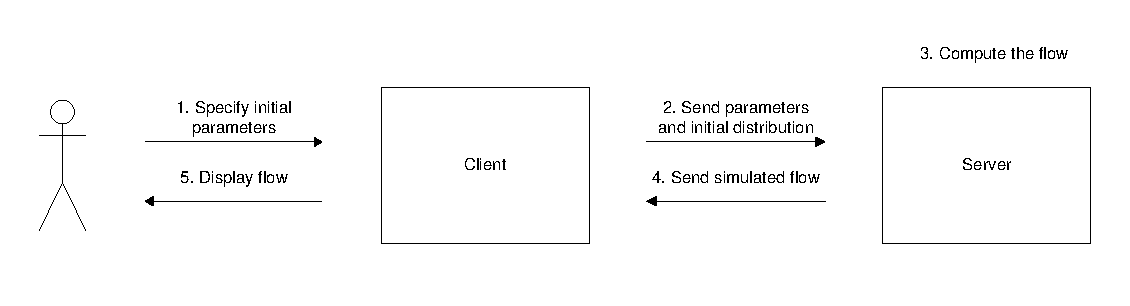
\includegraphics[width=\textwidth]{system-actor_diagram}\captionof{figure}{Domain model.\label{system-actor_diagram}}


\section{Assumptions and dependencies}
This section contains assumptions for the application to function properly.

\begin{itemize}
  \item As we are creating a client-server application, we assume that there is an internet connection between the client device and the server.
  \item As mentioned in the previous section, the application uses the \textsc{Fortran} implementation on the server to perform all the calculations. Therefore, we assume this server can compute the new concentration distribution correctly.
\end{itemize}

\noindent The following assumptions are in place to achieve our desired average time goals (see Section \ref{sec_constrReq} -- Requirements regarding performance).

\begin{itemize}
  \item We assume that the server can compute the calculations to compute the new concentration distribution within half a second.
  \item We assume that the communication between the client and the server can be handled within one second.
\end{itemize}
